\documentclass[serif]{beamer}
\usefonttheme{professionalfonts}
\usepackage{fontspec}
\setromanfont{Linux Libertine O}
\usepackage{mathtools}
%\usepackage{unicode-math}
% check name of font for your system, this works on Ubuntu
%\setmathfont{TeX Gyre Pagella Math}
\usepackage{ctexcap}
\usepackage{beamerthemesplit}
\usepackage{verbatim}
\usepackage{graphicx}
\usepackage{color}
\usepackage{xcolor}
\usepackage{leftidx}
\usepackage{bbold}
\usepackage{multicol}
\definecolor{darkgreen}{rgb}{0,73,52}
\definecolor{lightgreen}{rgb}{96,255,114}
\usetheme{Warsaw}
\setmainfont{Latin Modern Sans}
\CTEXoptions[today=old]
\begin{document}

\title{Deep Joint-Semantics Reconstructing Hashing for Large-Scale Unsupervised Cross-Modal Retrieval}
\author[Shupeng Su, Meire Fortunato] % (optional, use only with lots of authors)
{Oriol Vinyals\inst{1} \and Zhisheng Zhong\inst{2}}
% - Give the names in the same order as the appear in the paper.
% - Use the \inst{?} command only if the authors have different affiliation.
\institute[Beijing Institute of Technology] % (optional, but mostly needed)
{
  \inst{1}
  Key Laboratory of Machine Perception (MOE), School of EECS, Peking University
  \and
  \inst{2}
  Key Laboratory of Machine Perception (MOE), School of EECS, Peking University
}
\date{}
\frame{\titlepage}

\begin{frame}{Unsupervised Cross-Modal Retrieval}
\emph{Cross-Modal Retrieval}
\begin{figure}
    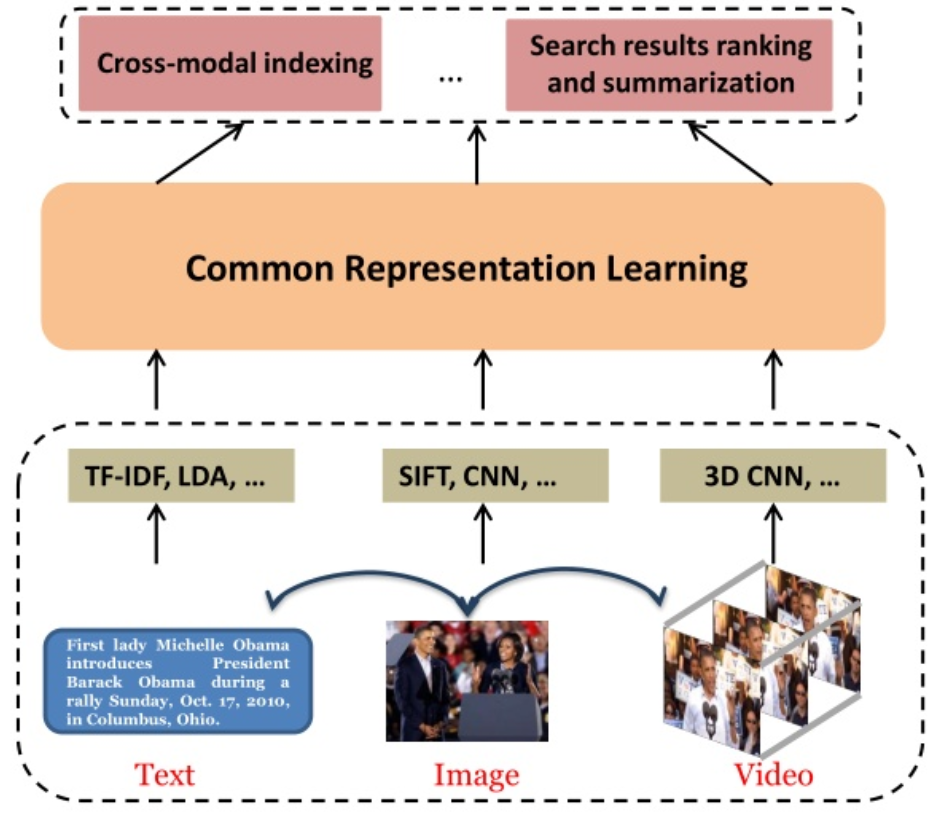
\includegraphics[height=5cm]{2.PNG}
\end{figure}
\emph{Binary representation learning}

\emph{Unsupervised Cross-Modal Retrieval}
\end{frame}

\begin{frame}{DJSRH}
\emph{Contributions}
\begin{itemize}
	\item Put forward affinity matrix.
	\item Reconstruct above jointsemantics, friendly for batch-wise training.
	\item Reach good result.
\end{itemize}
\end{frame}

\begin{frame}{DJSRH}
\begin{figure}
    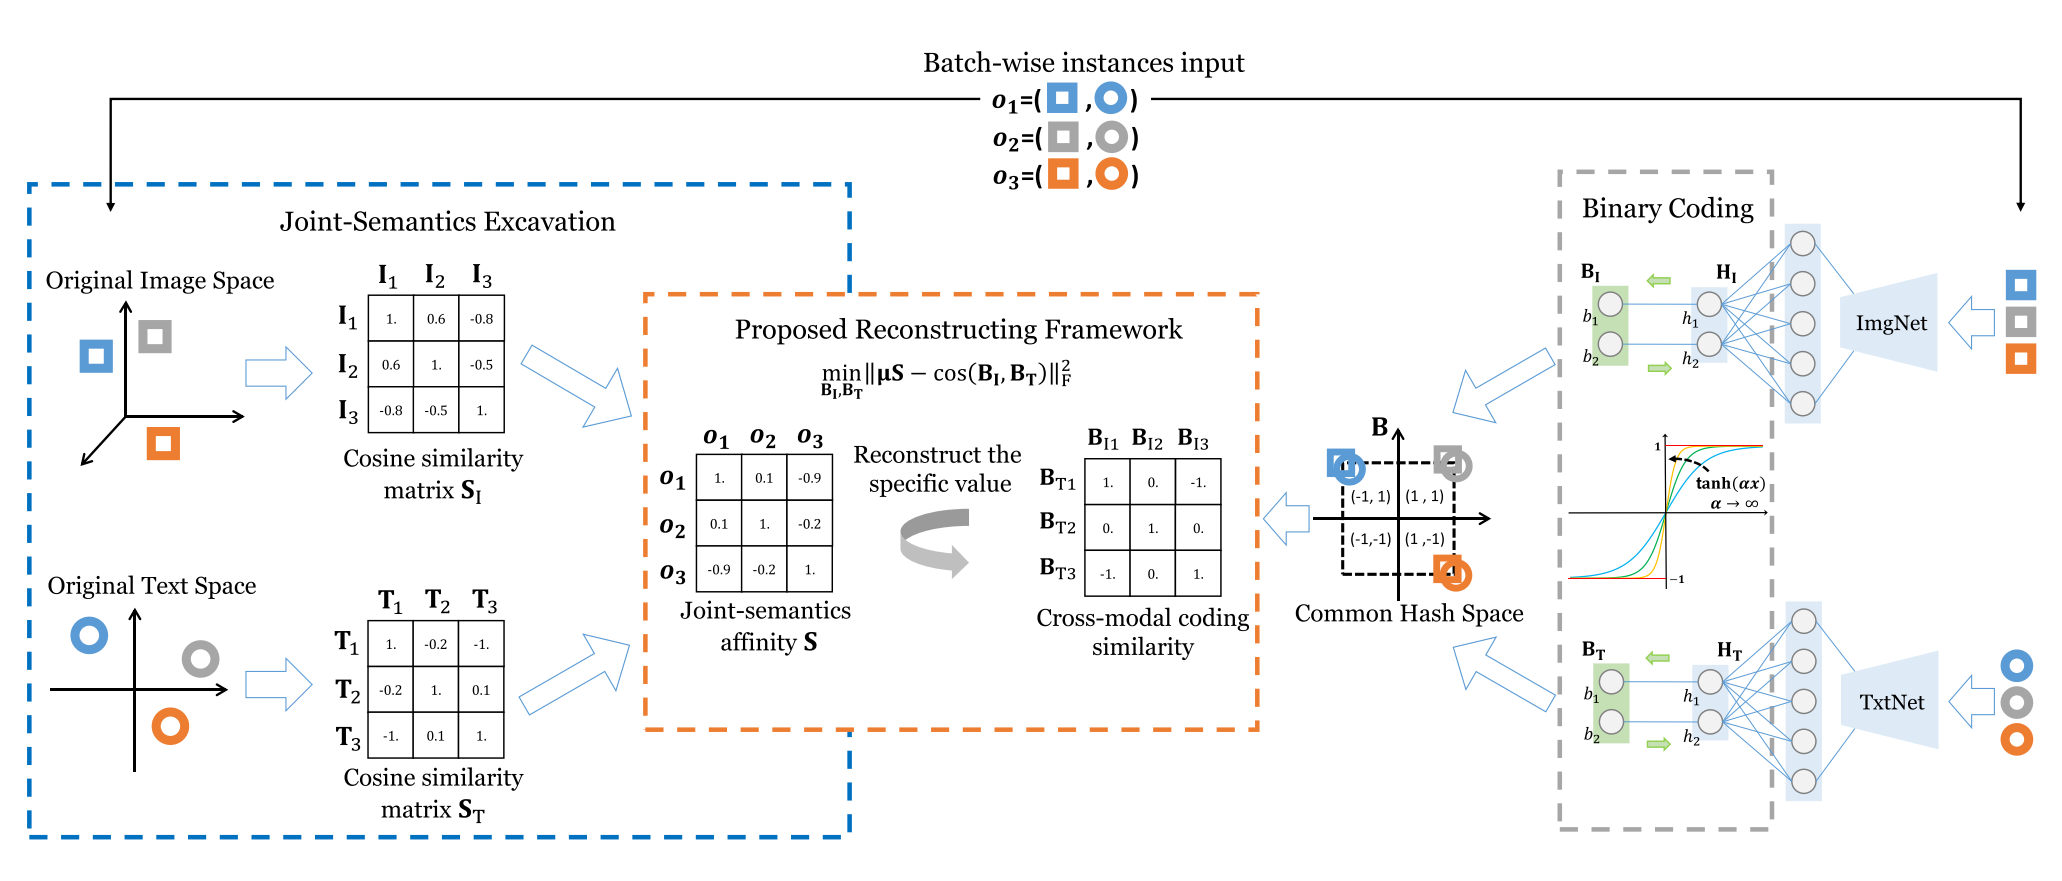
\includegraphics[height=4.5cm]{3.PNG}
	\caption{The pipeline of DJSRH}
\end{figure}
\end{frame}

\begin{frame}{Defination}
\begin{itemize}
 \item $m$: Batch size;
 \item $\mathcal{O}$: $\{o_k = \lceil \mathrm{I}_k, \mathrm{T}_k \rfloor\}_{k = 1}^m$, include each image-text pair. Feature matrix of image and text are defined as  $\mathrm{F}_\mathrm{I} \in \mathbb{R}^{m \times p_I}$ and $\mathrm{F}_\mathrm{T} \in \mathbb{R}^{m \times p_T}$;
 \item $\mathrm{B}_\mathrm{I} \in \{\pm1\}^{m\times d}$ and $\mathrm{B}_\mathrm{T} \in \{\pm1\}^{m\times d}$: Binary repesentation given out by ImgNet and TxtNet from the input $\mathrm{I}_k$ and $\mathrm{T}_k$;
 \item $\hat{\mathrm{F}}_\mathrm{I}$ and $\hat{\mathrm{F}}_\mathrm{T}$:The normalized $\mathrm{F}_\mathrm{I}$ and $\mathrm{F}_\mathrm{T}$,the cosine similarity matrices
$$
\mathrm{S}_\mathrm{I} = \hat{\mathrm{F}}_\mathrm{I}\hat{\mathrm{F}}_\mathrm{I}^\top \in [-1, +1]^{m \times m} 
$$
$$
\mathrm{S}_\mathrm{T} = \hat{\mathrm{F}}_\mathrm{T}\hat{\mathrm{F}}_\mathrm{T}^\top \in [-1, +1]^{m \times m}
$$
\end{itemize}
\end{frame}

\begin{frame}{Constructing Joint-Semantics Matrix}
\emph{Laplacian constrains}
$$
\min_{\mathrm{B}} \beta \mathrm{Tr}(\mathrm{B}^\top\mathrm{L_I}\mathrm{B}) + (1 - \beta)\mathrm{Tr}(\mathrm{B}^\top\mathrm{L_T}\mathrm{B})~~~\mathrm{s.t.}~ \mathrm{B} \in \{\pm1\}^{m \times d}
$$
where
$$
\mathrm{L_I} = \mathrm{diag}(\mathrm{S_11}) - \mathrm{S_I}
$$
$$
\mathrm{L_T} = \mathrm{diag}(\mathrm{S_T1}) - \mathrm{S_T}
$$
are Laplacian matrices.
\end{frame}

\begin{frame}{Constructing Joint-Semantics Matrix}
\emph{Joint-semantics Affinity Matrix}

Define $\mathcal{C}$ as combination function, then
$$
\mathrm{S} = \mathcal{C}(\mathrm{S_I}, \mathrm{S_T}) \in [-1, +1]^{m \times m}
$$

Merge Img and Txt as
$$
\tilde{\mathrm{S}} = \beta \mathrm{S_I} + (1 - \beta) \mathrm{S_T}
$$

Then
$$
\begin{aligned}
\mathrm{S} &= \mathcal{C}(\mathrm{S_I}, \mathrm{S_T}) \\
&= (1 - \eta) \tilde{\mathrm{S}} + \eta \frac{\tilde{\mathrm{S}}\tilde{\mathrm{S}}^\top}{m} \\
&= (1 - \eta)[\beta \mathrm{S_I} + (1 - \beta)\mathrm{S_T}] + \frac{\eta}{m}[\beta^2\mathrm{S_I}\mathrm{S_I}^\top + \beta(1 - \beta)(\mathrm{S_I}\mathrm{S_T}^\top + \mathrm{S_T}\mathrm{S_I}^\top) + (1 - \beta^2)\mathrm{S_T}\mathrm{S_T}^\top]
\end{aligned}
$$

$\mathrm{S}_{ij}$ indicates the latent semantic similarity between $o_i$ 和 $o_j$.
\end{frame}

\begin{frame}{Reconstructing with Binary Codes}
\emph{Object}

$$
\min_{\mathrm{B_I},\mathrm{B_T}} || \mu\mathrm{S} - \cos(\mathrm{B_I}, \mathrm{B_T})||_\mathrm{F}^2, ~~~\mathrm{s.t.}~ \mathrm{S} = \mathcal{C}(\mathrm{S_I}, \mathrm{S_T}) \in [-1, +1]^{m \times m}
$$

\emph{Laplacian constrains}
$$
\mathrm{Tr}(\mathrm{B}^\top\mathrm{L}\mathrm{B}) = \sum_{i, j} \mathrm{S}_{ij} ||\mathrm{B}_i - \mathrm{B}_j||^2
$$

\emph{Object with intra-modal influence}
$$
\begin{aligned}
\min_{\mathrm{B_I},\mathrm{B_T}} || \mu\mathrm{S} - \cos(\mathrm{B_I}, \mathrm{B_T})||_\mathrm{F}^2 + \lambda_1 || \mu\mathrm{S} - \cos(\mathrm{B_I}, \mathrm{B_I})||_\mathrm{F}^2 \\
+ \lambda_2 || \mu\mathrm{S} - \cos(\mathrm{B_T}, \mathrm{B_T})||_\mathrm{F}^2, \\ 
\mathrm{s.t.}~ \mathrm{S} = \mathcal{C}(\mathrm{S_I}, \mathrm{S_T}) \in [-1, +1]^{m \times m},~ \mathrm{B_I}, \mathrm{B_T} \in  \{-1, +1\}^{m \times d} 
\end{aligned}
$$
\end{frame}

\begin{frame}{Optimization}
Set $\mathrm{H} \in \mathbb{R}^{m \times d}$ as the last layer of ImgNet and TxtNet without activate function, then
$$
\mathrm{B} = \mathrm{sgn}(\mathrm{H}) \in \{-1, +1\}^{m \times d}
$$

Use the following instead,
$$
\mathrm{B} = \mathrm{tanh}(\alpha\mathrm{H}) \in \{-1, +1\}^{m \times d},~ \alpha \in \mathbb{R}^+
$$
\end{frame}

\begin{frame}{Algorithm}
\begin{figure}
    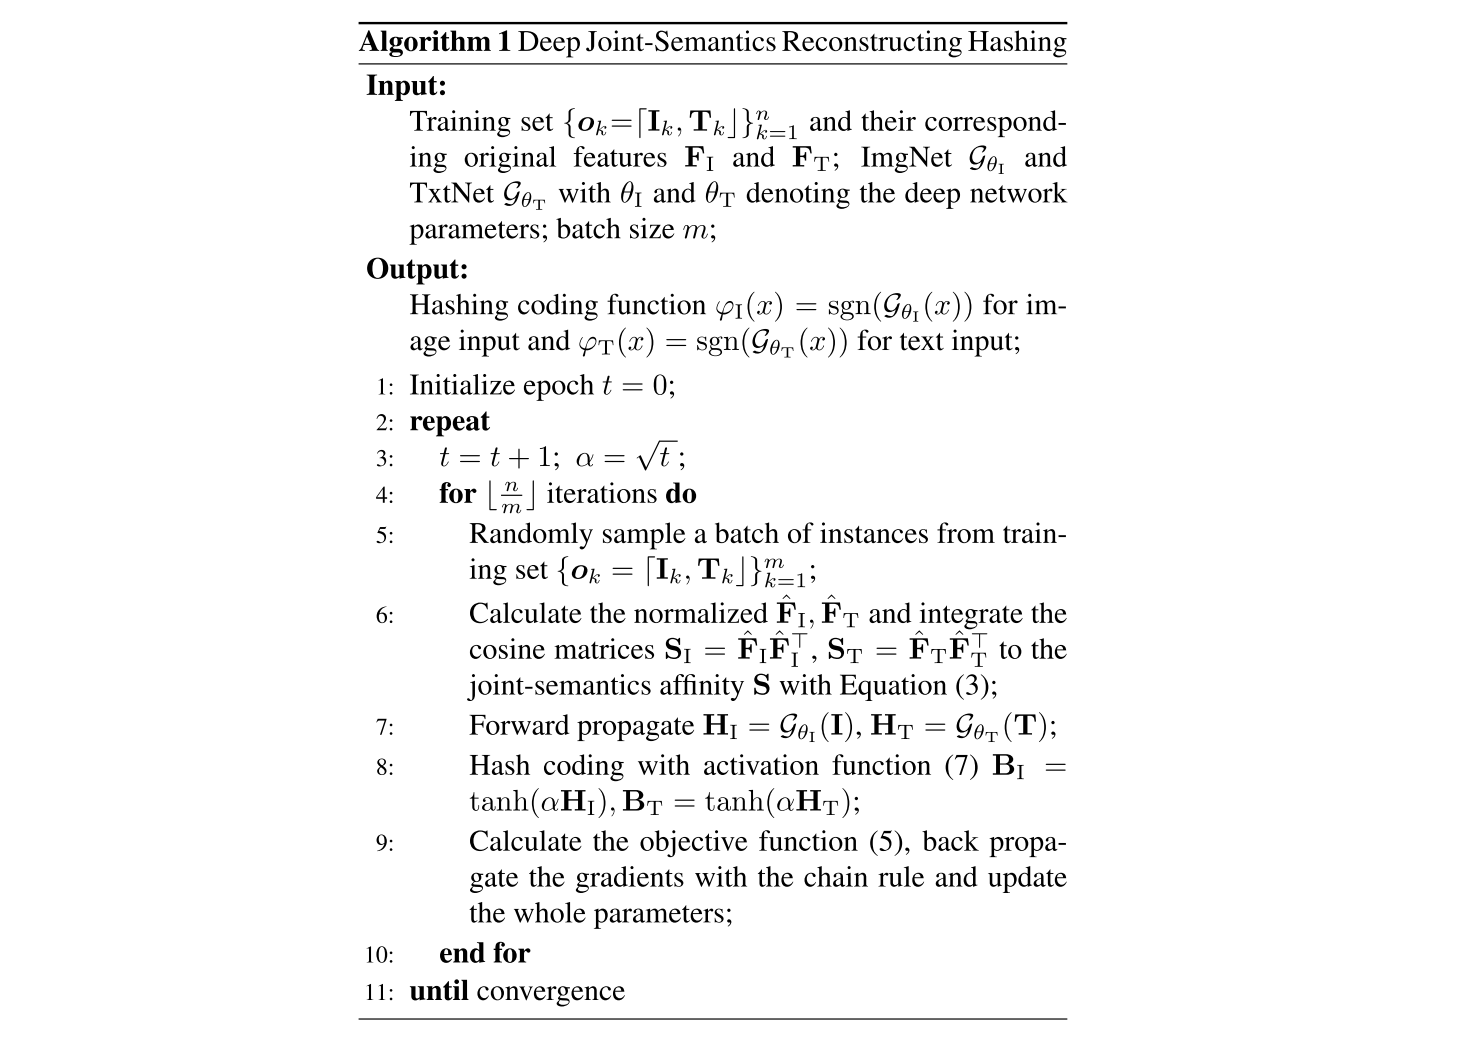
\includegraphics[height=7.5cm]{1.PNG}
\end{figure}
\end{frame}

\begin{frame}{Algorithm}
\begin{figure}
    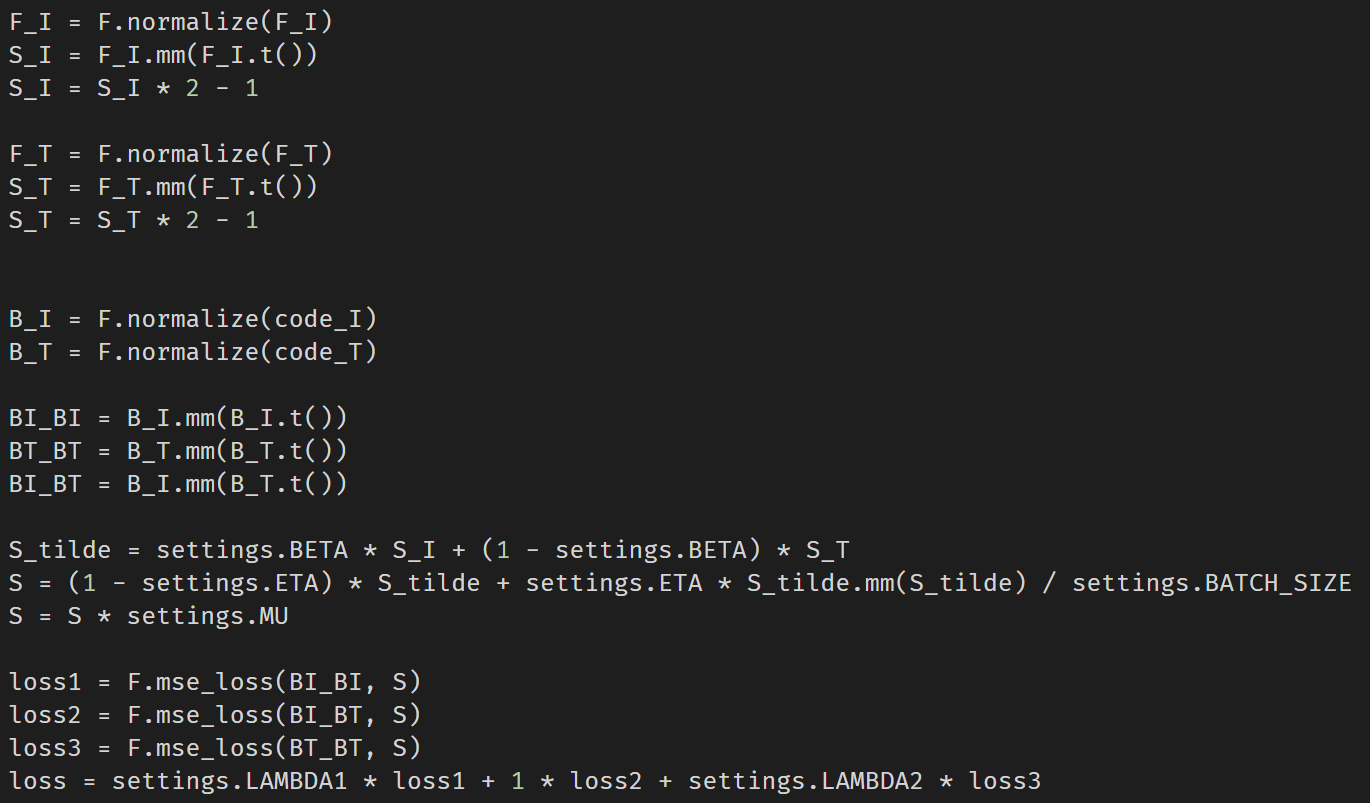
\includegraphics[height=6cm]{4.PNG}
\end{figure}
\end{frame}

\begin{frame}{Experiment}
\begin{figure}
    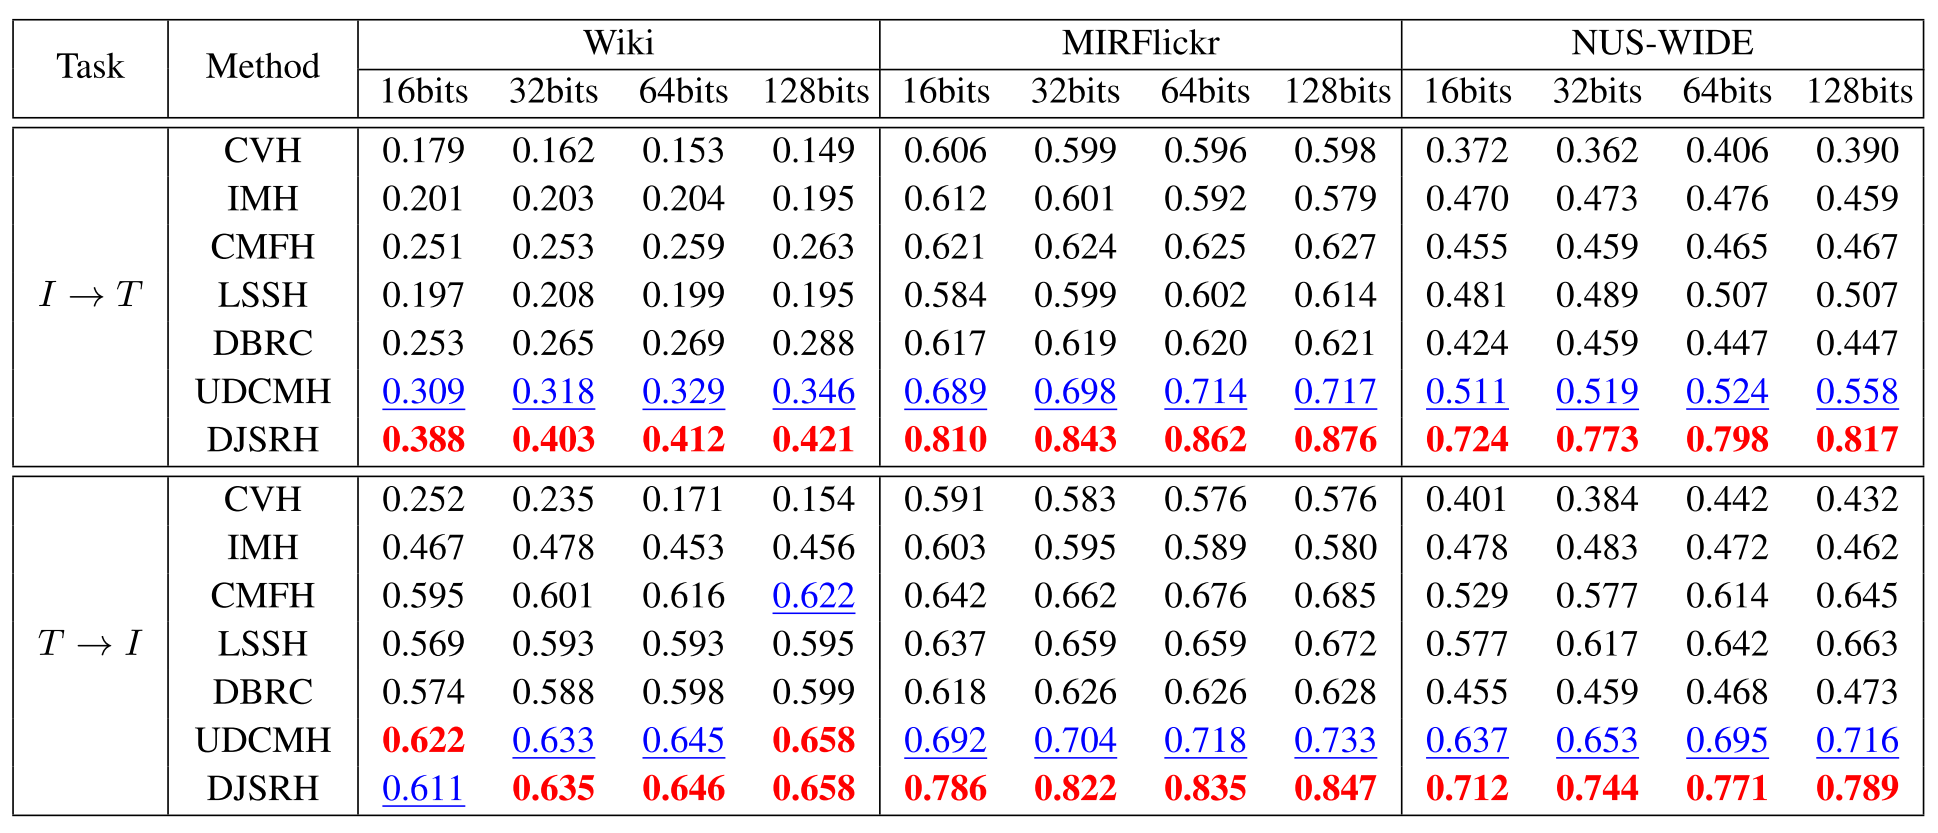
\includegraphics[height=5cm]{5.PNG}
	\caption{mAP@50}
\end{figure}
\end{frame}

\begin{frame}{Experiment}
MIRFlickr, CODELEN = 64
\begin{itemize}
	\item mAP of Image to Text: 0.865
	\item mAP of Text to Image: 0.853
\end{itemize}
\end{frame}

\end{document}
